\documentclass{article}
\usepackage[utf8]{inputenc}
\usepackage{tikz}

\usetikzlibrary{shapes.geometric, arrows}

\tikzstyle{start} = [circle, minimum width = 1cm, minimum height = 1cm, text centered, draw = black, fill = red!30]
\tikzstyle{stop} = [circle, minimum width = 1cm, minimum height = 1cm, text centered, draw = black, fill = red!30]
\tikzstyle{input} = [trapezium, trapezium left angle = 110, trapezium right angle = 110, minimum width = 1cm, minimum height = 1cm, text centered, draw = black, fill = cyan!30]
\tikzstyle{output} = [trapezium, trapezium left angle = 70, trapezium right angle = 70, minimum width = 1cm, minimum height = 1cm, text centered, draw = black, fill = cyan!30]
\tikzstyle{process} = [rectangle, minimum width = 3cm, minimum height = 1cm, text centered, draw = black, fill = yellow!30]
\tikzstyle{decision} = [diamond, minimum width = 2cm, minimum height = 1cm, text centered, draw = black, fill = green!30]
\tikzstyle{arrow} = [thick, ->, >=stealth]

\begin{document}
\begin{center}
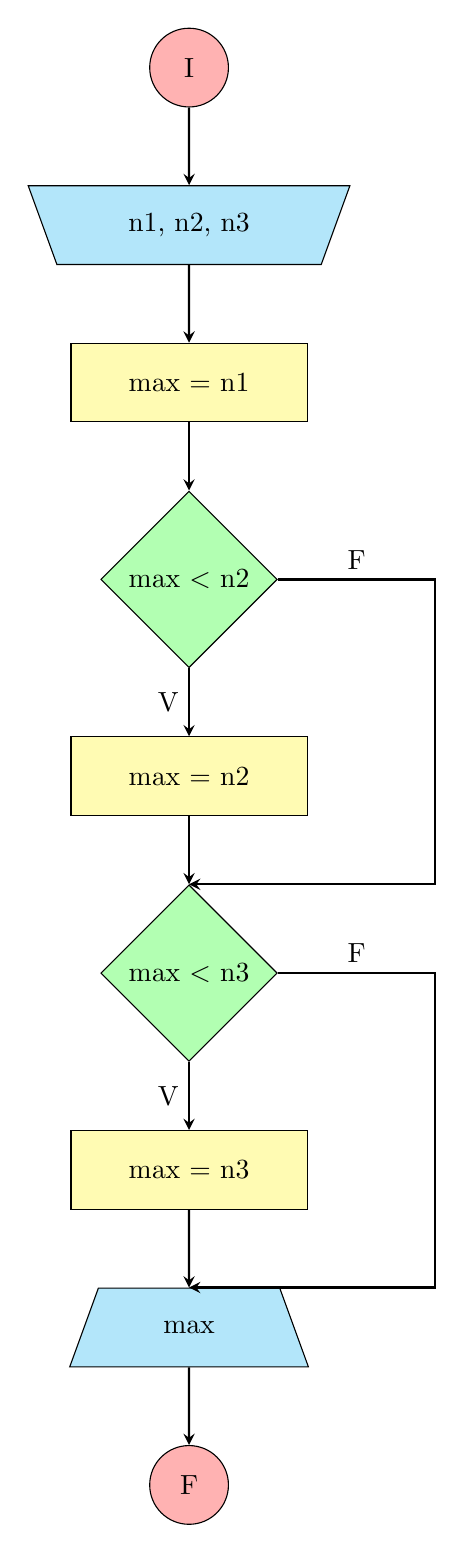
\begin{tikzpicture}[node distance = 2cm]
    \node(start1)[start]{I};
    \node(in1)[input, below of = start1]{n1, n2, n3};
    \node(pr1)[process, below of = in1]{max = n1};
    \node(dec1)[decision, below of = pr1, yshift = -0.5cm]{max $<$ n2};
    \node(pr2)[process, below of = dec1, yshift = -0.5cm]{max = n2};
    \node(dec2)[decision, below of = pr2, yshift = -0.5cm]{max $<$ n3};
    \node(pr3)[process, below of = dec2, yshift = -0.5cm]{max = n3};
    \node(out1)[output, below of = pr3]{max};
    \node(stop1)[stop, below of = out1]{F};

    \draw[arrow](start1)--(in1);
    \draw[arrow](in1)--(pr1);
    \draw[arrow](pr1)--(dec1);
    \draw[arrow](dec1)--node[anchor=east]{V}(pr2);
    \draw[arrow](dec1.east)--++(2,0)node[midway,above]{F}|-(dec2.north);
    \draw[arrow](pr2)--(dec2);
    \draw[arrow](dec2)--node[anchor=east]{V}(pr3);
    \draw[arrow](dec2.east)--++(2,0)node[midway,above]{F}|-(out1.north);
    \draw[arrow](pr3)--(out1);
    \draw[arrow](out1)--(stop1);
\end{tikzpicture}
\end{center}
\end{document}